% Chapter 2
\chapter{Models based on Quasi-Likelihood Estimation}

\fancyhead[RO,LE]{\thepage}
\fancyhead[LO]{Chapter 2 - \emph{Title of chapter}}
\fancyhead[RE]{Section \thesection \ - \emph{\Sectionname}}

\setlength{\parskip}{0.5pt}

\bigskip

\section{Quasi-likelihood inference} 
\noindent

\section{Quasi-likelihood function}
\noindent

\subsection{}
\noindent


\subsection{Title of subsection}
\noindent


\subsection{Title of subsection}
\noindent

\begin{figure}[!h]\centering
	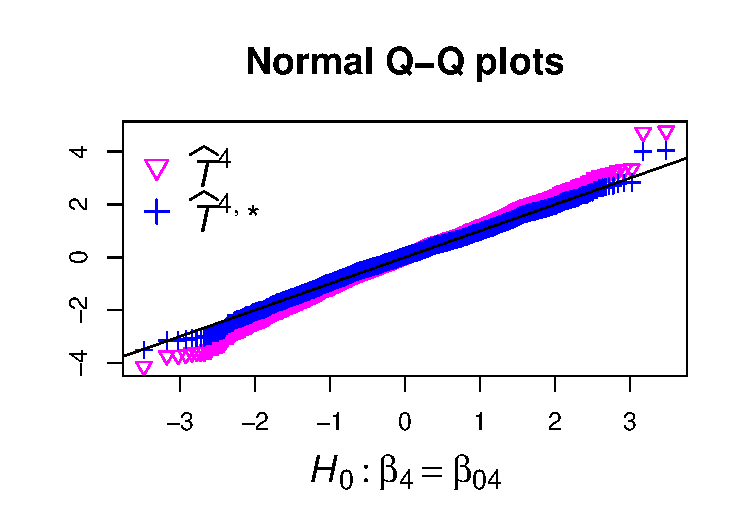
\includegraphics[width=12cm]{qq-clot.pdf}
	
	\caption{\label{qq-clot}Normal Q-Q plots based on 2000 values of $\widehat{T}^4$ and $\widehat{T}^{4,*}$ computed under the null hypothesis $H_0\!:\beta_4=\beta_{04}$ in the \emph{clotting} example.}
\end{figure}

\section{Generalized Estimating Equations}
\noindent